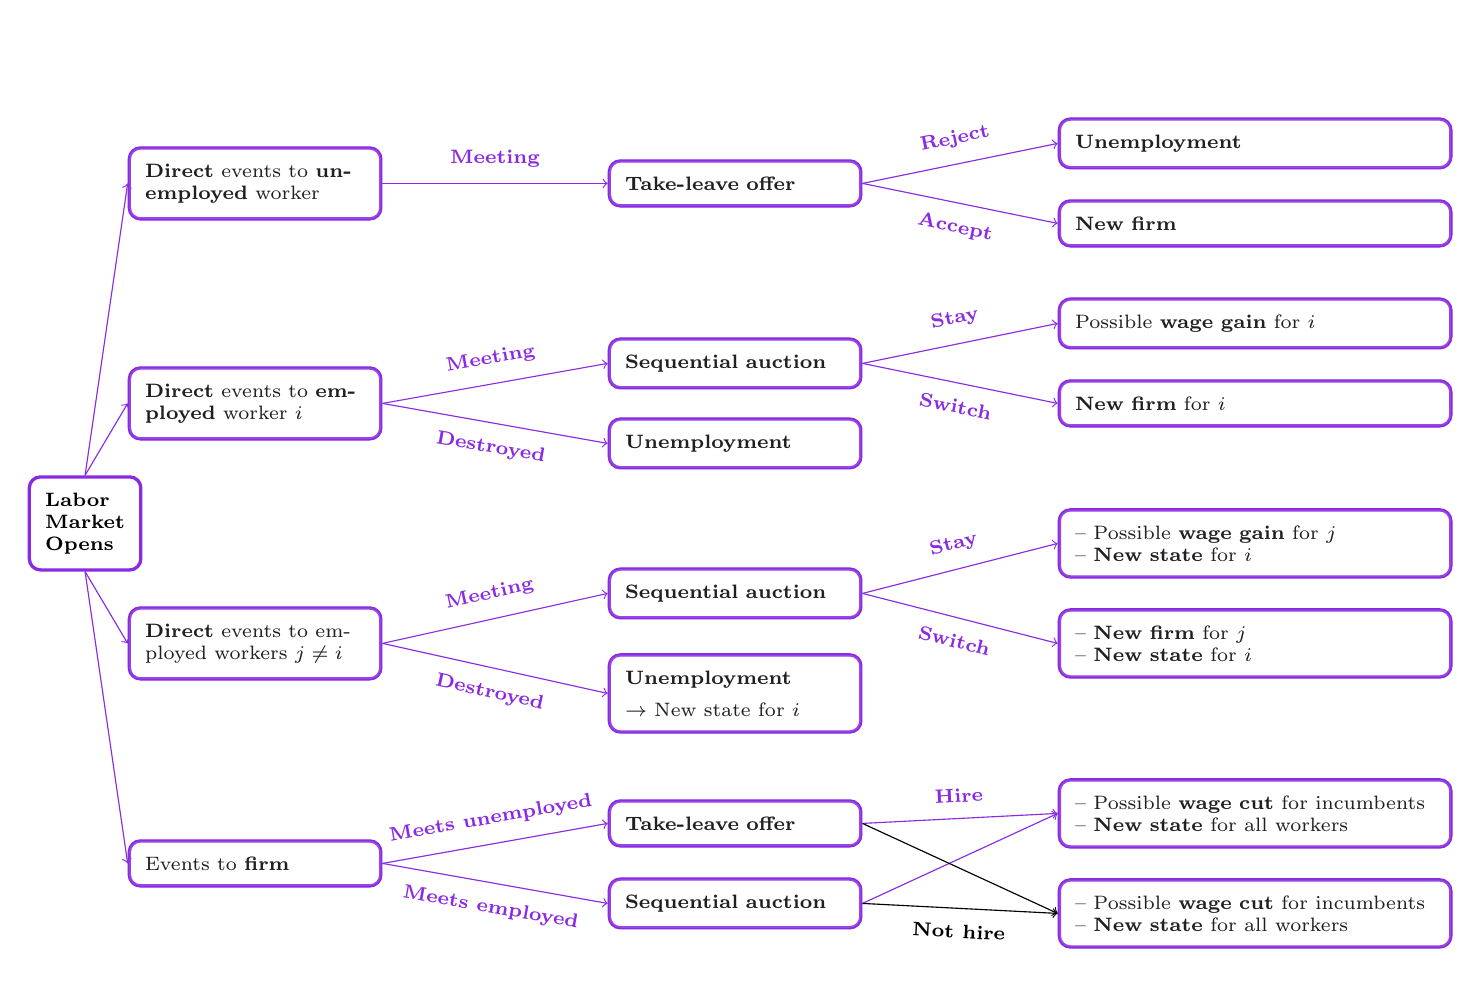
\begin{tikzpicture}[
    grow=right,
    kant/.style={text width=4cm, text centered, sloped},
    every node/.style={text ragged, inner sep=2mm},
    punkt/.style={rectangle, rounded corners, %shade, top color=white,
    %bottom color=blue!50!black!20
    , draw=BlueViolet, very thick}
    , font=\scriptsize
    ]
% first row
\node[punkt, text width=.4in,fill=white] (init) {\alert{\textbf{Labor Market Opens}} \\};
%\alt<1,6->{\node[punkt, text width=.7in,fill=white] (init) {\alert{\textbf{Labor Market Opens}}};}{\node[punkt, black, text width=.7in, opacity=0.15] (init) {Labor Market Opens};}

% second row
\node[text width=0in, right of=init, node distance = .85in] (init2) {};
\node [text width=0in, above of=init2, node distance=2.4in] {};
\node [text width=0in, below of=init2, node distance=2.2in] {};


% 1ST BRANCH

\node[punkt, text width=1.1in, above of=init2, node distance = 1.7in, fill=white] (unemployed1) {\textbf{\alert{Direct}} events to \textbf{\alert{unemployed}} worker};
\draw[->,BlueViolet] (init.north) -- (unemployed1.west) {};

\node [punkt, text width=1.1in, right of=unemployed1, node distance=2.4in,fill=white] (unemployed2) {\textbf{\alert{Take-leave offer}}};
\draw[->,BlueViolet] (unemployed1) -- (unemployed2) node[midway,above,sloped] {\textbf{\alertroyalblue{Meeting}}};

\node [text width=0in, right of=unemployed2, node distance=2.6in] (unemployed3) {};
\node [punkt, text width=1.8in, opacity=1, above of=unemployed3, node distance=.2in, fill=white] (unemployed31) {\textbf{\alert{Unemployment}}};
\draw[->,opacity=1,BlueViolet] (unemployed2.east) -- (unemployed31.west) node[midway,above,sloped,opacity=1] {\textbf{\alertroyalblue{Reject}}};
\node [punkt, text width=1.8in, opacity=1, below of=unemployed3, node distance=.2in, fill=white] (unemployed32) {\textbf{\alert{New firm}}};
\draw[->,opacity=1,BlueViolet] (unemployed2.east) -- (unemployed32.west) node[midway,below,sloped,opacity=1] {\textbf{\alertroyalblue{Accept}}};



\node[punkt, text width=1.1in, above of=init2, node distance = 1.7in, fill=white, opacity=0.15] (unemployed1) {\textbf{\alert{Direct}} events to \textbf{\alert{unemployed}} worker};
\draw[->,BlueViolet, opacity=0.15] (init.north) -- (unemployed1.west) {};

\node [punkt, text width=1.1in, right of=unemployed1, node distance=2.4in,fill=white, opacity=0.15] (unemployed2) {\textbf{\alert{Take-leave offer}}};
\draw[->,BlueViolet, opacity=0.15] (unemployed1) -- (unemployed2) node[midway,above,sloped] {\textbf{\alertroyalblue{Meeting}}};

\node [text width=0in, right of=unemployed2, node distance=2.6in] (unemployed3) {};
\node [punkt, text width=1.8in, above of=unemployed3, node distance=.2in, fill=white, opacity=0.15] (unemployed31) {\textbf{\alert{Unemployment}}};
\draw[->,BlueViolet, opacity=0.15] (unemployed2.east) -- (unemployed31.west) node[midway,above,sloped, opacity=0.15] {\textbf{\alertroyalblue{Reject}}};
\node [punkt, text width=1.8in, below of=unemployed3, node distance=.2in, fill=white, opacity=0.15] (unemployed32) {\textbf{\alert{New firm}}};
\draw[->,BlueViolet, opacity=0.15] (unemployed2.east) -- (unemployed32.west) node[midway,below,sloped, opacity=0.15] {\textbf{\alertroyalblue{Accept}}};



% 2ND BRANCH

\node [punkt, text width=1.1in, above of=init2, node distance = .6in, fill=white] (employed1) {\textbf{\alert{Direct}} events to \textbf{\alert{employed}} worker \alert{$\pmb{i}$}};
\draw[->,BlueViolet] (init.north) -- (employed1.west) {};

\node [text width=0in, right of=employed1, node distance=2.4in] (employed2) {};
\node [punkt, text width=1.1in, above of=employed2, node distance=.2in,fill=white] (employed21) {\textbf{\alert{Sequential auction}}};
\draw[->,BlueViolet] (employed1.east) -- (employed21.west) node[midway,above,sloped] {\textbf{\alertroyalblue{Meeting}}};
\node [punkt, text width=1.1in, below of=employed2, node distance=.2in,fill=white] (employed22) {\textbf{\alert{Unemployment}}};
\draw[->,BlueViolet] (employed1.east) -- (employed22.west) node[midway,below,sloped] {\textbf{\alertroyalblue{Destroyed}}};

\node [text width=0in, right of=employed21, node distance=2.6in] (employed3) {};
\node [punkt, text width=1.8in, opacity=1, above of=employed3, node distance=.2in, fill=white] (employed31) {Possible \textbf{\alert{wage gain}} for \alert{$\pmb{i}$}};
\draw[->,opacity=1,BlueViolet] (employed21.east) -- (employed31.west) node[midway,above,sloped,opacity=1] {\textbf{\alertroyalblue{Stay}}};
\node [punkt, text width=1.8in, opacity=1, below of=employed3, node distance=.2in, fill=white] (employed32) {\textbf{\alert{New firm}} for \alert{$\pmb{i}$}};
\draw[->,opacity=1,BlueViolet] (employed21.east) -- (employed32.west) node[midway,below,sloped,opacity=1] {\textbf{\alertroyalblue{Switch}}};


\node [punkt, text width=1.1in, above of=init2, node distance = .6in, fill=white, opacity=0.15] (employed1) {\textbf{\alert{Direct}} events to \textbf{\alert{employed}} worker \alert{$\pmb{i}$}};
\draw[->,BlueViolet, opacity=0.15] (init.north) -- (employed1.west) {};

\node [text width=0in, right of=employed1, node distance=2.4in, opacity=0.15] (employed2) {};
\node [punkt, text width=1.1in, above of=employed2, node distance=.2in,fill=white, opacity=0.15] (employed21) {\textbf{\alert{Sequential auction}}};
%\draw[->,BlueViolet, opacity=0.15] (employed1.east) -- (employed21.west) node[midway,above,sloped] {\textbf{\alertroyalblue{Contact}}};
\node [punkt, text width=1.1in, below of=employed2, node distance=.2in,fill=white, opacity=0.15] (employed22) {\textbf{\alert{Unemployment}}};
\draw[->,BlueViolet, opacity=0.15] (employed1.east) -- (employed22.west) node[midway,below,sloped] {\textbf{\alertroyalblue{Destroyed}}};

\node [text width=0in, right of=employed21, node distance=2.6in, opacity=0.15] (employed3) {};
\node [punkt, text width=1.8in, above of=employed3, node distance=.2in, fill=white, opacity=0.15] (employed31) {Possible \textbf{\alert{wage gain}} for \alert{$\pmb{i}$}};
\draw[->,BlueViolet, opacity=0.15] (employed21.east) -- (employed31.west) node[midway,above,sloped, opacity=0.15] {\textbf{\alertroyalblue{Stay}}};
\node [punkt, text width=1.8in, below of=employed3, node distance=.2in, fill=white, opacity=0.15] (employed32) {\textbf{\alert{New firm}} for \alert{$\pmb{i}$}};
\draw[->,opacity=1,BlueViolet, opacity=0.15] (employed21.east) -- (employed32.west) node[midway,below,sloped, opacity=0.15] {\textbf{\alertroyalblue{Switch}}};



% 3RD BRANCH

\node [punkt, text width=1.1in, below of=init2, node distance = 0.6in, fill=white] (indirect1) {\textbf{\alert{Direct}} events to employed workers \alert{$\pmb{j \neq i}$}};
\draw[->,BlueViolet] (init.south) -- (indirect1.west) {};

\node [text width=0in, right of=indirect1, node distance=2.4in] (indirect2) {};
\node [punkt, text width=1.1in, above of=indirect2, node distance=.25in,fill=white] (indirect21) {\textbf{\alert{Sequential auction}}};
\draw[->,BlueViolet] (indirect1.east) -- (indirect21.west) node[midway,above,sloped] {\textbf{\alertroyalblue{Meeting}}};
\node [punkt, text width=1.1in, below of=indirect2, node distance=.25in,fill=white] (indirect22) {\textbf{\alert{Unemployment}} \\[.05in]
$\rightarrow$ New state for \alert{$\pmb{i}$}};
\draw[->,BlueViolet] (indirect1.east) -- (indirect22.west) node[midway,below,sloped] {\textbf{\alertroyalblue{Destroyed}}};

\node [text width=0in, right of=indirect21, node distance=2.6in] (indirect3) {};
\node [punkt, text width=1.8in, opacity=1, above of=indirect3, node distance=.25in, fill=white] (indirect31) {-- Possible \textbf{\alert{wage gain}} for \alert{$\pmb{j}$} \\
-- \textbf{\alert{New state}} for \alert{$\pmb{i}$}};
\draw[->,BlueViolet] (indirect21.east) -- (indirect31.west) node[midway,above,sloped,opacity=1] {\textbf{\alertroyalblue{Stay}}};
\node [punkt, text width=1.8in, below of=indirect3, node distance=.25in, fill=white] (indirect32) {-- \textbf{\alert{New firm}} for \alert{$\pmb{j}$} \\
-- \textbf{\alert{New state}} for \alert{$\pmb{i}$}};
\draw[->,BlueViolet] (indirect21.east) -- (indirect32.west) node[midway,below,sloped,opacity=1] {\textbf{\alertroyalblue{Switch}}};


\node [punkt, text width=1.1in, below of=init2, node distance = 0.6in, fill=white, opacity=0.15] (indirect1) {\textbf{\alert{Direct}} events to employed workers \alert{$\pmb{j \neq i}$}};
\draw[->,BlueViolet, opacity=0.15] (init.south) -- (indirect1.west) {};

\node [text width=0in, right of=indirect1, node distance=2.4in, opacity=0.15] (indirect2) {};
\node [punkt, text width=1.1in, above of=indirect2, node distance=.25in,fill=white, opacity=0.15] (indirect21) {\textbf{\alert{Sequential auction}}};
%\draw[->,BlueViolet, opacity=0.15] (indirect1.east) -- (indirect21.west) node[midway,above,sloped] {\textbf{\alertroyalblue{Contact}}}
\node [punkt, text width=1.1in, below of=indirect2, node distance=.25in,fill=white, opacity=0.15] (indirect22) {\textbf{\alert{Unemployment}} \\[.05in]
$\rightarrow$ New state for \alert{$\pmb{i}$}};
\draw[->,BlueViolet, opacity=0.15] (indirect1.east) -- (indirect22.west) node[midway,below,sloped] {\textbf{\alertroyalblue{Destroyed}}};

\node [text width=0in, right of=indirect21, node distance=2.6in, opacity=0.15] (indirect3) {};
\node [punkt, text width=1.8in, above of=indirect3, node distance=.25in, fill=white, opacity=0.15] (indirect31) {-- Possible \textbf{\alert{wage gain}} for \alert{$\pmb{j}$} \\
-- \textbf{\alert{New state}} for \alert{$\pmb{i}$}};
\draw[->,BlueViolet, opacity=0.15] (indirect21.east) -- (indirect31.west) node[midway,above,sloped, opacity=0.15] {\textbf{\alertroyalblue{Stay}}};
\node [punkt, text width=1.8in, below of=indirect3, node distance=.25in, fill=white, opacity=0.15] (indirect32) {-- \textbf{\alert{New firm}} for \alert{$\pmb{j}$} \\
-- \textbf{\alert{New state}} for \alert{$\pmb{i}$}};
\draw[->,BlueViolet, opacity=0.15] (indirect21.east) -- (indirect32.west) node[midway,below,sloped, opacity=0.15] {\textbf{\alertroyalblue{Switch}}};


% 4TH BRANCH

\node [punkt, text width=1.1in, below of=init2, node distance=1.7in, fill=white](firm1){Events to \textbf{\alert{firm}}};
\draw[->,BlueViolet] (init.south) -- (firm1.west) {};

\node [text width=0in, right of=firm1, node distance=2.4in] (firm2) {};
\node [punkt, text width=1.1in, above of=firm2, node distance=.2in,fill=white] (firm21) {\textbf{\alert{Take-leave offer}}};
\draw[->,BlueViolet] (firm1.east) -- (firm21.west) node[midway,above,sloped] {\textbf{\alertroyalblue{Meets unemployed}}};
\node [punkt, text width=1.1in, below of=firm2, node distance=.2in,fill=white] (firm22) {\textbf{\alert{Sequential auction}}};
\draw[->,BlueViolet] (firm1.east) -- (firm22.west) node[midway,below,sloped] {\textbf{\alertroyalblue{Meets employed}}};

\node [text width=0in, right of=firm2, node distance=2.6in] (firm3) {};
\node [punkt, text width=1.8in, opacity=1, above of=firm3, node distance=.25in, fill=white] (firm31) {-- Possible \textbf{\alert{wage cut}} for incumbents \\
-- \textbf{\alert{New state}} for all workers};
\node [punkt, text width=1.8in, opacity=1, below of=firm3, node distance=.25in, fill=white] (firm32) {-- Possible \textbf{\alert{wage cut}} for incumbents \\
-- \textbf{\alert{New state}} for all workers};
\draw[->,opacity=1,BlueViolet] (firm21.east) -- (firm31.west) node[midway,above,sloped,opacity=1] { \textbf{\alertroyalblue{Hire}}};
\draw[->,opacity=1,BlueViolet] (firm22.east) -- (firm31.west) node[midway,above,sloped,opacity=1] {};
\draw[->,opacity=1] (firm21.east) -- (firm32.west) node[midway,below,sloped,opacity=1] {};
\draw[->,opacity=1] (firm22.east) -- (firm32.west) node[midway,below,sloped,opacity=1] {\textbf{\alert{Not hire}}};


\node [punkt, text width=1.1in, below of=init2, node distance=1.7in, fill=white, opacity=0.15](firm1){Events to \textbf{\alert{firm}}};
\draw[->,BlueViolet, opacity=0.15] (init.south) -- (firm1.west) {};

\node [text width=0in, right of=firm1, node distance=2.4in] (firm2) {};
\node [punkt, text width=1.1in, above of=firm2, node distance=.2in,fill=white, opacity=0.15] (firm21) {\textbf{\alert{Take-leave offer}}};
\draw[->,BlueViolet, opacity=0.15] (firm1.east) -- (firm21.west) node[midway,above,sloped] {\textbf{\alertroyalblue{Meets unemployed}}};
\node [punkt, text width=1.1in, below of=firm2, node distance=.2in,fill=white, opacity=0.15] (firm22) {\textbf{\alert{Sequential auction}}};
\draw[->,BlueViolet, opacity=0.15] (firm1.east) -- (firm22.west) node[midway,below,sloped] {\textbf{\alertroyalblue{Meets employed}}};

\node [text width=0in, right of=firm2, node distance=2.6in] (firm3) {};
\node [punkt, text width=1.8in, above of=firm3, node distance=.25in, fill=white, opacity=0.15] (firm31) {-- Possible \textbf{\alert{wage cut}} for incumbents \\
-- \textbf{\alert{New state}} for all workers};
\node [punkt, text width=1.8in, below of=firm3, node distance=.25in, fill=white, opacity=0.15] (firm32) {-- Possible \textbf{\alert{wage cut}} for incumbents \\
-- \textbf{\alert{New state}} for all workers};
\draw[->,BlueViolet, opacity=0.15] (firm21.east) -- (firm31.west) node[midway,above,sloped, opacity=0.15] {\textbf{\alertroyalblue{Hire}}};
\draw[->,BlueViolet, opacity=0.15] (firm22.east) -- (firm31.west) node[midway,above,sloped, opacity=0.15] {};
\draw[->, opacity=0.15] (firm21.east) -- (firm32.west) node[midway,below,sloped, opacity=0.15] {};
\draw[->, opacity=0.15] (firm22.east) -- (firm32.west) node[midway,below,sloped, opacity=0.15] {\textbf{\alert{Not hire}}};


\end{tikzpicture}
